\section{Primer prototipo: Generación de modelos Django mediante CodeT5}
\label{sec:primer-prototipo}

\subsection{Herramientas y tecnologías utilizadas}
\label{subsec:p1-herramientas}

Para el primer prototipo se utilizaron diferentes herramientas orientadas al análisis del lenguaje \textit{Idioms}, la construcción de su representación semántica y la generación automática de código para Django ORM. Las principales tecnologías empleadas fueron las siguientes:

\begin{itemize}
    \item \textbf{Python:} Lenguaje principal para la implementación del procesamiento, generación de datos, entrenamiento del modelo y ejecución del prototipo.
    \item \textbf{TypeScript:} Utilizado para la implementación de componentes encargados de procesar la información obtenida a partir del análisis del lenguaje \textit{Idioms} y construir la representación semántica. En particular, se desarrolló el componente \texttt{CodeT5InputBuilder.ts}, encargado de recorrer la estructura sintáctica generada por ANTLR4 y construir un modelo semántico compuesto por entidades, atributos, identificadores y relaciones.
    \item \textbf{ANTLR4:} Empleado para el análisis léxico y sintáctico del lenguaje \textit{Idioms}, permitiendo procesar los modelos definidos mediante el DSL y obtener una estructura susceptible de ser transformada.
    \item \textbf{Django ORM:} Tecnología de destino para representar mediante código Python las entidades y relaciones definidas en los modelos de \textit{Idioms}.
    \item \textbf{CodeT5:} Modelo de lenguaje basado en la arquitectura T5, utilizado para realizar la transformación de la representación semántica hacia código de modelos Django.
    \item \textbf{Hugging Face Transformers:} Biblioteca utilizada para cargar, ajustar y ejecutar el modelo CodeT5.
    \item \textbf{PyTorch:} \textit{Framework} de aprendizaje automático para el entrenamiento y ejecución del modelo.
    \item \textbf{JSON:} Formato estructurado para almacenar la representación semántica generada a partir del modelo definido en \textit{Idioms} y como entrada para la generación de código.
\end{itemize}

La interacción entre estas tecnologías permitió establecer el flujo general del primer prototipo, partiendo de un modelo expresado en \textit{Idioms} y finalizando con la generación de un archivo \texttt{models.py}.

\subsection{Construcción de la representación semántica}
\label{subsec:p1-representacion-semantica}

Como parte del desarrollo del primer prototipo, se estableció una representación semántica intermedia que permitiera separar el análisis del lenguaje \textit{Idioms} del proceso posterior de generación de código. Esta representación organizó la información obtenida en una estructura independiente del lenguaje de programación de destino.

El proceso inicia con la definición de un modelo utilizando la sintaxis de \textit{Idioms}. Este es procesado mediante ANTLR4 para realizar el análisis léxico y sintáctico. A partir de este procesamiento se desarrolló el componente \texttt{CodeT5InputBuilder.ts} en TypeScript, el cual extiende el \textit{listener} generado por ANTLR4 y recorre el Árbol Sintáctico Abstracto (\textit{AST}).

La información obtenida es posteriormente serializada en formato JSON en el archivo \texttt{semantic.json} (véase Anexo~\ref{anx:codigo-builder}), estructurado principalmente en dos componentes: \texttt{entities} y \texttt{relations}. Un ejemplo simplificado de esta representación se muestra a continuación:

\begin{verbatim}
{
  "language": "Django",
  "entities": [
    {
      "name": "User",
      "attributes": [
        { "name": "name", "type": "string" }
      ]
    },
    {
      "name": "Country",
      "attributes": [
        { "name": "name", "type": "string" }
      ]
    }
  ],
  "relations": [
    {
      "type": "classification",
      "from": "User",
      "to": "Country",
      "role": "nationality"
    }
  ]
}
\end{verbatim}

\subsection{Preparación de la entrada para CodeT5}
\label{subsec:p1-preparacion-entrada}

Una vez obtenida la representación semántica, el componente \texttt{CodeT5InputBuilder.ts} transformó esta información en ejemplos estructurados para el entrenamiento del modelo.

De manera general, el proceso de preparación siguió el siguiente flujo:
\begin{figure}[htbp]
    \centering
    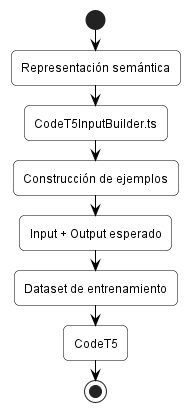
\includegraphics[width=0.22\textwidth]{diagramas/preparacion_datos_codet5/preparacion_datos_codet5.png}
    \caption{Flujo general del proceso de preparación de datos para CodeT5.}
    \label{fig:preparacion-datos-codet5}
\end{figure}

El flujo de conversión empaquetó las estructuras en pares de instrucción, entrada semántica y salida esperada en Django ORM (Anexo~\ref{anx:dataset-ejemplo}):

\begin{verbatim}
{
  "instruction": "Generate Django ORM models from semantic representation.",
  "input": "{ ... representación semántica JSON ... }",
  "output": "from django.db import models\n\nclass User(models.Model): ..."
}
\end{verbatim}

\subsection{Evaluación inicial y ajuste de CodeT5}
\label{subsec:p1-evaluacion-ajuste}

Inicialmente se realizó una evaluación \textit{zero-shot} utilizando el modelo preentrenado \texttt{Salesforce/codet5-base} sin ningún ajuste específico (Anexo~\ref{anx:prueba-zeroshot}). El flujo inicial de experimentación fue el siguiente: 
\begin{figure}[htbp]
    \centering
    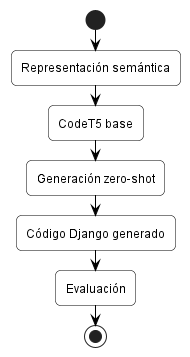
\includegraphics[width=0.22\textwidth]{diagramas/flujo_zero_shot/flujo_zero_shot.png}
    \caption{Flujo inicial de experimentación mediante generación \textit{zero-shot}.}
    \label{fig:flujo-zero-shot}
\end{figure}

Se observó que, aunque el modelo contaba con conocimientos generales de código, presentaba inconsistencias para interpretar la semántica propia de \textit{Idioms}.

Por este motivo, se realizó un proceso de \textit{fine-tuning} (Anexo~\ref{anx:script-entrenamiento}) entrenándolo con el conjunto de datos preparado. Como resultado se obtuvo la versión base ajustada denominada \textbf{V4}. Posteriormente, se realizaron experimentos de ajuste incremental generando las versiones \textbf{V4.1} y \textbf{V4.2} para estudiar estrategias frente a múltiples relaciones.
\begin{figure}[htbp]
    \centering
    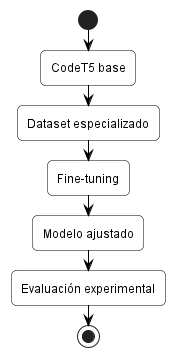
\includegraphics[width=0.25\textwidth]{diagramas/flujo_fine_tuning/flujo_fine_tuning.png}
    \caption{Flujo empleado para el ajuste fino (\textit{fine-tuning}) y evaluación experimental del modelo.}
    \label{fig:flujo-fine-tuning}
\end{figure}

\subsection{Validación del primer prototipo}
\label{subsec:p1-validacion}

La validación concentró su análisis en relaciones del \textit{idiom} ``clasificación'' para establecer escenarios controlados (Anexo~\ref{anx:casos-prueba}). Se evaluó la capacidad de traducir entidades, atributos y la correcta asignación de origen, destino y rol en las relaciones. Se implementó un script de evaluación automatizada (Anexo~\ref{anx:script-evaluacion}) para seleccionar rangos de prueba y calcular la precisión.

\subsection{Resultados de la evaluación del primer prototipo}
\label{subsec:p1-resultados}

Mientras que la generación de entidades y atributos alcanzó un comportamiento satisfactorio, la generación de relaciones fue inestable. A continuación se resumen los resultados obtenidos en las diferentes iteraciones:

\begin{itemize}
    \item \textbf{Versión V4:} Evaluada en pequeños rangos de prueba; en un bloque de 4 casos con relaciones alcanzó el $50{,}00\%$ de precisión (2 correctos), y en un bloque de 6 casos descendió al $16{,}67\%$ (1 correcto).
    \item \textbf{Versión V4.1:} Sobre 29 ejemplos con relaciones, logró 20 casos correctos y 9 incorrectos, alcanzando la mayor precisión con un \textbf{$68{,}97\%$}.
    \item \textbf{Versión V4.2:} Diseñada para reforzar escenarios de 2 y 3 relaciones; sobre 11 ejemplos únicamente 1 fue correcto, cayendo a un \textbf{$9{,}09\%$} de precisión.
\end{itemize}

En la Cuadro~\ref{tab:comparativa-versiones} se sintetiza la evaluación comparativa entre las versiones.

\begin{table}[htbp]
\centering
\caption{Comparativa general de precisión en la generación de relaciones (Prototipo 1).}
\label{tab:comparativa-versiones}
\begin{tabular}{lcccc}
\hline
\textbf{Versión} & \textbf{Casos Evaluados} & \textbf{Correctos} & \textbf{Incorrectos} & \textbf{Precisión} \\ \hline
V4 (Muestra A)   & 4                        & 2                  & 2                    & $50{,}00\%$       \\
V4 (Muestra B)   & 6                        & 1                  & 5                    & $16{,}67\%$       \\
V4.1             & 29                       & 20                 & 9                    & \textbf{68,97\%}  \\
V4.2             & 11                       & 1                  & 10                   & $9{,}09\%$        \\ \hline
\end{tabular}
\end{table}

\subsection{Limitaciones identificadas en el primer prototipo}
\label{subsec:p1-limitaciones}

Las principales fallas identificadas en la generación neuronal con CodeT5 fueron:
\begin{enumerate}
    \item \textbf{Omisión de relaciones:} En modelos con múltiples relaciones, CodeT5 tendía a ignorar la segunda o tercera relación.
    \item \textbf{Asignación incorrecta de atributos/relaciones:} Asignaba la clave foránea a una entidad distinta de la especificada en el JSON.
    \item \textbf{Alucinación de relaciones:} Creación de relaciones inexistentes en la entrada.
    \item \textbf{Falta de mejora por sobre-entrenamiento:} La versión V4.2 demostró que aumentar ejemplos relacionales no resuelve la falta de determinismo del modelo neuronal.
\end{enumerate}

Esta limitación fundamentó la necesidad de diseñar la **Arquitectura Híbrida del Prototipo 2** (planteada en el Capítulo III), donde las entidades y atributos se delegan a CodeT5 pero las relaciones son procesadas mediante un algoritmo determinístico.